%!TEX TS-program = xelatex

\documentclass {article}

\usepackage{xetexko}
\usepackage[a4paper]{geometry}
\usepackage[usenames,dvipsnames]{xcolor}
\usepackage{mathtools}
\usepackage{amsmath}
\usepackage{fontspec}
\usepackage{hyperref}
\usepackage{graphicx}
\usepackage{listings}
\usepackage{makeidx}
\usepackage{indentfirst}
\usepackage{tikz}
\usetikzlibrary{arrows,automata}


%\setmainfont {NanumMyeongjo}
\setmainfont {UnBatang}
\setmonofont[Scale=0.8]{DejaVu Sans Mono}

\lstdefinestyle{diff}{
  belowcaptionskip=1\baselineskip,
  breaklines=true,
  frame=L,
  xleftmargin=\parindent,
  showstringspaces=false,
  % Diffstart
  morecomment=[f][\color{gray}]{@@},
  % Diffincl
  morecomment=[f][\color{Green}]{+},
  % Diffrem
  morecomment=[f][\color{Red}]{-},
  basicstyle=\footnotesize\ttfamily,
}

\lstdefinestyle{customtxt}{
  belowcaptionskip=1\baselineskip,
  breaklines=true,
  frame=L,
  xleftmargin=\parindent,
  showstringspaces=false,
  basicstyle=\footnotesize\ttfamily,
}

\lstdefinestyle{customc}{
  belowcaptionskip=1\baselineskip,
  breaklines=true,
  frame=L,
  xleftmargin=\parindent,
  language=C,
  showstringspaces=false,
  basicstyle=\footnotesize\ttfamily,
  keywordstyle=\bfseries\color{green!40!black},
  commentstyle=\itshape\color{purple!40!black},
  identifierstyle=\color{blue},
  stringstyle=\color{orange},
}

\lstdefinestyle{customrs}{
  belowcaptionskip=1\baselineskip,
  breaklines=true,
  frame=L,
  xleftmargin=\parindent,
  showstringspaces=false,
  morekeywords={fn,let,mut,pub,use,impl,struct,unsafe,if,for},
  morecomment=[l]{//},
  morecomment=[n]{/*}{*/},
  basicstyle=\footnotesize\ttfamily,
  keywordstyle=\bfseries\color{green!40!black},
  commentstyle=\itshape\color{purple!40!black},
  identifierstyle=\color{blue},
  stringstyle=\color{orange},
}


\begin {document}

\title {OS 3차 과제 - 가상메모리의 이해와 procfs 를 통한 분석}
\input {../../reportauthor.tex}
\maketitle

% Requirement: Mark Wss change
% Poll measurement 500msec.
% Display process during 1 sec when Wss changed.

\section {리눅스의 Paging}
리눅스는 가상 메모리를 3단계 페이징 기법(AMD64 시스템과, 몇몇 ARM 시스템은 4단계)을 통해 물리 프레임으로 매핑한다. 여기에서 모든 가상 메모리가 리얼 메모리로 매핑되어야 할 필요는 없는데, 이를 이용한 페이징 기법이 Demanded paging 이다. 이는 프로세스가 요청한 모든 가상 메모리를 프레임에 매핑하지 않고, 실제 데이터를 접근할 때, 페이지를 프레임에 할당하는 방식으로 메인 메모리와 secondary storage 를 활용하여 물리 메모리의 요구량을 줄이게 된다.
\section {Working set}
주어진 시간동안 프로세스가 필요로 하는 메모리를 Working set 이라 한다. Working set 은 프로세스가 실행되는 과정에서 바뀌게 되며, 적당한 시간 간격을 잡으면, working set 은 Locality 를 나타내게 된다. 이는 working set 에 해당하는 메모리들이 해당되는 window 동안 메모리에 남아 있다면, 프로세스는 페이지 폴트를 처리할 필요 없이 진행할 수 있다.
\section {Thrashing}
Demanded paging 을 사용하는 시스템은 프로그램 전체를 메모리에 올리지 않고, secondary storage 에서 필요할 때마다 필요한 page 를 이동시키게 된다. 만약, 이 때 시스템의 메모리가 프로세스가 필요로 하는 Working set size 보다 작다면, 프로세스는 연산을 진행하면 지속적으로 Working set 에 포함된 데이터가 secondary storage 로 스왑되게 된다. 이는 지속적인 페이지 폴트를 유발, Page fault handler 가 secondary storage 로 이동된 프레임을 다시 메모리로 불러오게 되고, 이는 CPU의 활용율을 낮추게 된다.

이 페이지 폴트를 처리하는 시간이 프로그램이 실제로 실행되는 시간보다 길어지게 되면, 이를 Thrashing 이라고 한다 
\section {Swap partition}
페이지 폴트를 처리하기 위해 메모리를 할당해야하지만, 남은 프레임이 없을 경우엔, victim frame 을 정해서 이를 secondary storage 로 옮기고, victim frame 이 있던 프레임에 요청된 데이터를 로드하게 된다. 이 과정에 쓰이는 secondary storage 공간이 스왑 파티션이다.
\section {코드 설명}
테스트 환경:
OS: Gentoo Linux
C Compiler: GCC 4.9.2 with --std=gnu99
Make: GNU Make 4.1

작성한 프로그램은 /proc/[pid]/statm 파일을 일정 주기 (여기서는 0.5초) 마다 읽어와서, 파싱한 뒤, 결과를 보여주도록 작성되었습니다.
더불어 /proc/[pid]/comm 파일에서 프로세스의 이름을 가져와 로깅 파일 이름과, 화면 표시에 사용되도록 작성되었습니다.
\lstinputlisting [style=customc]{project/procmon.c}
\lstinputlisting [style=customc]{project/procmon.h}
\lstinputlisting [style=customc]{project/getmemstat.c}
\lstinputlisting [style=customc]{project/getmemstat.h}

\section {실행 결과 분석}
\subsection {프로그램 실행 사진}
\begin {figure}[h]
  \centering
  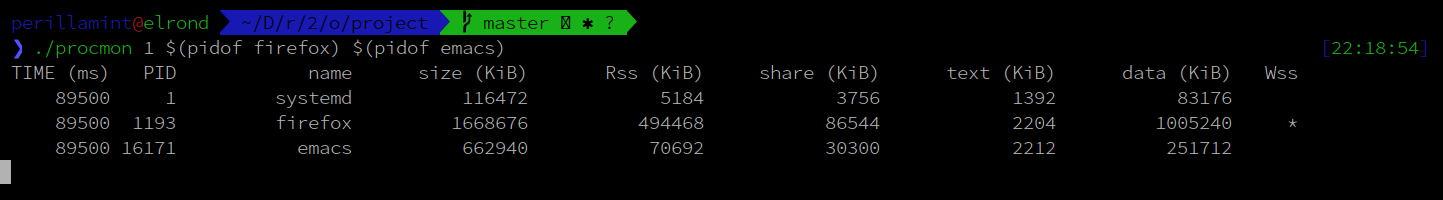
\includegraphics [width=120mm]{screenshot.png}
  \caption {실행 스크린샷}
  \label{fig:systemd}
\end {figure}

\newpage
\subsection{백그라운드 프로세스 - systemd (init)}
시스템에서 systemd는 시스템을 초기화하고 데몬을 시동하는 역활을 한다. 이에서 일상적 상황(데몬 재시동 요청이 없는 상황) 에서는 systemd 는 백그라운드에 sleep 상태로 머무르게 됨을 의미한다. 따라서 systemd 의 메모리 소모량은 측정 시간 동안 크게 변하지 않을 것을 예상할 수 있고, 결과도 추측과 같게 나온다.

\begin {figure}[h]
  \centering
  % GNUPLOT: LaTeX picture with Postscript
\begingroup
  \makeatletter
  \providecommand\color[2][]{%
    \GenericError{(gnuplot) \space\space\space\@spaces}{%
      Package color not loaded in conjunction with
      terminal option `colourtext'%
    }{See the gnuplot documentation for explanation.%
    }{Either use 'blacktext' in gnuplot or load the package
      color.sty in LaTeX.}%
    \renewcommand\color[2][]{}%
  }%
  \providecommand\includegraphics[2][]{%
    \GenericError{(gnuplot) \space\space\space\@spaces}{%
      Package graphicx or graphics not loaded%
    }{See the gnuplot documentation for explanation.%
    }{The gnuplot epslatex terminal needs graphicx.sty or graphics.sty.}%
    \renewcommand\includegraphics[2][]{}%
  }%
  \providecommand\rotatebox[2]{#2}%
  \@ifundefined{ifGPcolor}{%
    \newif\ifGPcolor
    \GPcolortrue
  }{}%
  \@ifundefined{ifGPblacktext}{%
    \newif\ifGPblacktext
    \GPblacktextfalse
  }{}%
  % define a \g@addto@macro without @ in the name:
  \let\gplgaddtomacro\g@addto@macro
  % define empty templates for all commands taking text:
  \gdef\gplbacktext{}%
  \gdef\gplfronttext{}%
  \makeatother
  \ifGPblacktext
    % no textcolor at all
    \def\colorrgb#1{}%
    \def\colorgray#1{}%
  \else
    % gray or color?
    \ifGPcolor
      \def\colorrgb#1{\color[rgb]{#1}}%
      \def\colorgray#1{\color[gray]{#1}}%
      \expandafter\def\csname LTw\endcsname{\color{white}}%
      \expandafter\def\csname LTb\endcsname{\color{black}}%
      \expandafter\def\csname LTa\endcsname{\color{black}}%
      \expandafter\def\csname LT0\endcsname{\color[rgb]{1,0,0}}%
      \expandafter\def\csname LT1\endcsname{\color[rgb]{0,1,0}}%
      \expandafter\def\csname LT2\endcsname{\color[rgb]{0,0,1}}%
      \expandafter\def\csname LT3\endcsname{\color[rgb]{1,0,1}}%
      \expandafter\def\csname LT4\endcsname{\color[rgb]{0,1,1}}%
      \expandafter\def\csname LT5\endcsname{\color[rgb]{1,1,0}}%
      \expandafter\def\csname LT6\endcsname{\color[rgb]{0,0,0}}%
      \expandafter\def\csname LT7\endcsname{\color[rgb]{1,0.3,0}}%
      \expandafter\def\csname LT8\endcsname{\color[rgb]{0.5,0.5,0.5}}%
    \else
      % gray
      \def\colorrgb#1{\color{black}}%
      \def\colorgray#1{\color[gray]{#1}}%
      \expandafter\def\csname LTw\endcsname{\color{white}}%
      \expandafter\def\csname LTb\endcsname{\color{black}}%
      \expandafter\def\csname LTa\endcsname{\color{black}}%
      \expandafter\def\csname LT0\endcsname{\color{black}}%
      \expandafter\def\csname LT1\endcsname{\color{black}}%
      \expandafter\def\csname LT2\endcsname{\color{black}}%
      \expandafter\def\csname LT3\endcsname{\color{black}}%
      \expandafter\def\csname LT4\endcsname{\color{black}}%
      \expandafter\def\csname LT5\endcsname{\color{black}}%
      \expandafter\def\csname LT6\endcsname{\color{black}}%
      \expandafter\def\csname LT7\endcsname{\color{black}}%
      \expandafter\def\csname LT8\endcsname{\color{black}}%
    \fi
  \fi
    \setlength{\unitlength}{0.0500bp}%
    \ifx\gptboxheight\undefined%
      \newlength{\gptboxheight}%
      \newlength{\gptboxwidth}%
      \newsavebox{\gptboxtext}%
    \fi%
    \setlength{\fboxrule}{0.5pt}%
    \setlength{\fboxsep}{1pt}%
\begin{picture}(8640.00,3024.00)%
    \gplgaddtomacro\gplbacktext{%
      \csname LTb\endcsname%
      \put(990,440){\makebox(0,0)[r]{\strut{}$0$}}%
      \put(990,827){\makebox(0,0)[r]{\strut{}$20000$}}%
      \put(990,1213){\makebox(0,0)[r]{\strut{}$40000$}}%
      \put(990,1600){\makebox(0,0)[r]{\strut{}$60000$}}%
      \put(990,1986){\makebox(0,0)[r]{\strut{}$80000$}}%
      \put(990,2373){\makebox(0,0)[r]{\strut{}$100000$}}%
      \put(990,2759){\makebox(0,0)[r]{\strut{}$120000$}}%
      \put(1122,220){\makebox(0,0){\strut{}$0$}}%
      \put(1730,220){\makebox(0,0){\strut{}$20000$}}%
      \put(2338,220){\makebox(0,0){\strut{}$40000$}}%
      \put(2946,220){\makebox(0,0){\strut{}$60000$}}%
      \put(3554,220){\makebox(0,0){\strut{}$80000$}}%
      \put(4163,220){\makebox(0,0){\strut{}$100000$}}%
      \put(4771,220){\makebox(0,0){\strut{}$120000$}}%
      \put(5379,220){\makebox(0,0){\strut{}$140000$}}%
      \put(5987,220){\makebox(0,0){\strut{}$160000$}}%
      \put(6595,220){\makebox(0,0){\strut{}$180000$}}%
    }%
    \gplgaddtomacro\gplfronttext{%
      \csname LTb\endcsname%
      \put(7651,2649){\makebox(0,0)[r]{\strut{}size}}%
      \csname LTb\endcsname%
      \put(7651,2429){\makebox(0,0)[r]{\strut{}Rss}}%
      \csname LTb\endcsname%
      \put(7651,2209){\makebox(0,0)[r]{\strut{}shared}}%
    }%
    \gplbacktext
    \put(0,0){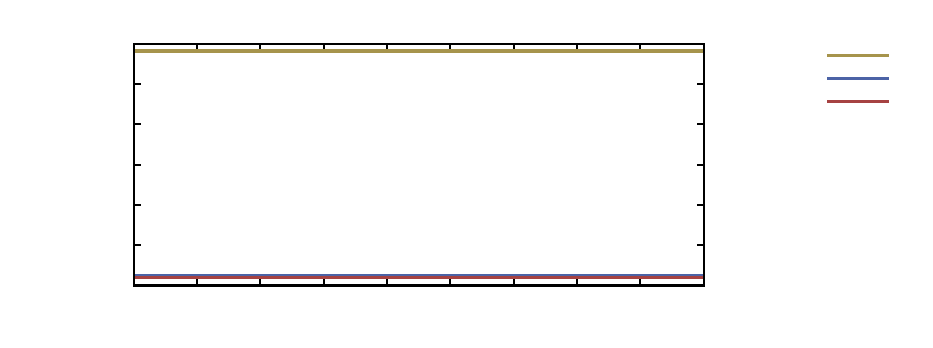
\includegraphics{memlog-systemd-with-vm}}%
    \gplfronttext
  \end{picture}%
\endgroup

  \caption {Systemd 의 메모리 기록}
  % GNUPLOT: LaTeX picture with Postscript
\begingroup
  \makeatletter
  \providecommand\color[2][]{%
    \GenericError{(gnuplot) \space\space\space\@spaces}{%
      Package color not loaded in conjunction with
      terminal option `colourtext'%
    }{See the gnuplot documentation for explanation.%
    }{Either use 'blacktext' in gnuplot or load the package
      color.sty in LaTeX.}%
    \renewcommand\color[2][]{}%
  }%
  \providecommand\includegraphics[2][]{%
    \GenericError{(gnuplot) \space\space\space\@spaces}{%
      Package graphicx or graphics not loaded%
    }{See the gnuplot documentation for explanation.%
    }{The gnuplot epslatex terminal needs graphicx.sty or graphics.sty.}%
    \renewcommand\includegraphics[2][]{}%
  }%
  \providecommand\rotatebox[2]{#2}%
  \@ifundefined{ifGPcolor}{%
    \newif\ifGPcolor
    \GPcolortrue
  }{}%
  \@ifundefined{ifGPblacktext}{%
    \newif\ifGPblacktext
    \GPblacktextfalse
  }{}%
  % define a \g@addto@macro without @ in the name:
  \let\gplgaddtomacro\g@addto@macro
  % define empty templates for all commands taking text:
  \gdef\gplbacktext{}%
  \gdef\gplfronttext{}%
  \makeatother
  \ifGPblacktext
    % no textcolor at all
    \def\colorrgb#1{}%
    \def\colorgray#1{}%
  \else
    % gray or color?
    \ifGPcolor
      \def\colorrgb#1{\color[rgb]{#1}}%
      \def\colorgray#1{\color[gray]{#1}}%
      \expandafter\def\csname LTw\endcsname{\color{white}}%
      \expandafter\def\csname LTb\endcsname{\color{black}}%
      \expandafter\def\csname LTa\endcsname{\color{black}}%
      \expandafter\def\csname LT0\endcsname{\color[rgb]{1,0,0}}%
      \expandafter\def\csname LT1\endcsname{\color[rgb]{0,1,0}}%
      \expandafter\def\csname LT2\endcsname{\color[rgb]{0,0,1}}%
      \expandafter\def\csname LT3\endcsname{\color[rgb]{1,0,1}}%
      \expandafter\def\csname LT4\endcsname{\color[rgb]{0,1,1}}%
      \expandafter\def\csname LT5\endcsname{\color[rgb]{1,1,0}}%
      \expandafter\def\csname LT6\endcsname{\color[rgb]{0,0,0}}%
      \expandafter\def\csname LT7\endcsname{\color[rgb]{1,0.3,0}}%
      \expandafter\def\csname LT8\endcsname{\color[rgb]{0.5,0.5,0.5}}%
    \else
      % gray
      \def\colorrgb#1{\color{black}}%
      \def\colorgray#1{\color[gray]{#1}}%
      \expandafter\def\csname LTw\endcsname{\color{white}}%
      \expandafter\def\csname LTb\endcsname{\color{black}}%
      \expandafter\def\csname LTa\endcsname{\color{black}}%
      \expandafter\def\csname LT0\endcsname{\color{black}}%
      \expandafter\def\csname LT1\endcsname{\color{black}}%
      \expandafter\def\csname LT2\endcsname{\color{black}}%
      \expandafter\def\csname LT3\endcsname{\color{black}}%
      \expandafter\def\csname LT4\endcsname{\color{black}}%
      \expandafter\def\csname LT5\endcsname{\color{black}}%
      \expandafter\def\csname LT6\endcsname{\color{black}}%
      \expandafter\def\csname LT7\endcsname{\color{black}}%
      \expandafter\def\csname LT8\endcsname{\color{black}}%
    \fi
  \fi
    \setlength{\unitlength}{0.0500bp}%
    \ifx\gptboxheight\undefined%
      \newlength{\gptboxheight}%
      \newlength{\gptboxwidth}%
      \newsavebox{\gptboxtext}%
    \fi%
    \setlength{\fboxrule}{0.5pt}%
    \setlength{\fboxsep}{1pt}%
\begin{picture}(8640.00,3024.00)%
    \gplgaddtomacro\gplbacktext{%
      \csname LTb\endcsname%
      \put(726,440){\makebox(0,0)[r]{\strut{}$3600$}}%
      \put(726,730){\makebox(0,0)[r]{\strut{}$3800$}}%
      \put(726,1020){\makebox(0,0)[r]{\strut{}$4000$}}%
      \put(726,1310){\makebox(0,0)[r]{\strut{}$4200$}}%
      \put(726,1600){\makebox(0,0)[r]{\strut{}$4400$}}%
      \put(726,1889){\makebox(0,0)[r]{\strut{}$4600$}}%
      \put(726,2179){\makebox(0,0)[r]{\strut{}$4800$}}%
      \put(726,2469){\makebox(0,0)[r]{\strut{}$5000$}}%
      \put(726,2759){\makebox(0,0)[r]{\strut{}$5200$}}%
      \put(858,220){\makebox(0,0){\strut{}$0$}}%
      \put(1525,220){\makebox(0,0){\strut{}$20000$}}%
      \put(2192,220){\makebox(0,0){\strut{}$40000$}}%
      \put(2858,220){\makebox(0,0){\strut{}$60000$}}%
      \put(3525,220){\makebox(0,0){\strut{}$80000$}}%
      \put(4192,220){\makebox(0,0){\strut{}$100000$}}%
      \put(4859,220){\makebox(0,0){\strut{}$120000$}}%
      \put(5525,220){\makebox(0,0){\strut{}$140000$}}%
      \put(6192,220){\makebox(0,0){\strut{}$160000$}}%
      \put(6859,220){\makebox(0,0){\strut{}$180000$}}%
    }%
    \gplgaddtomacro\gplfronttext{%
      \csname LTb\endcsname%
      \put(7651,2649){\makebox(0,0)[r]{\strut{}size}}%
      \csname LTb\endcsname%
      \put(7651,2429){\makebox(0,0)[r]{\strut{}Rss}}%
    }%
    \gplbacktext
    \put(0,0){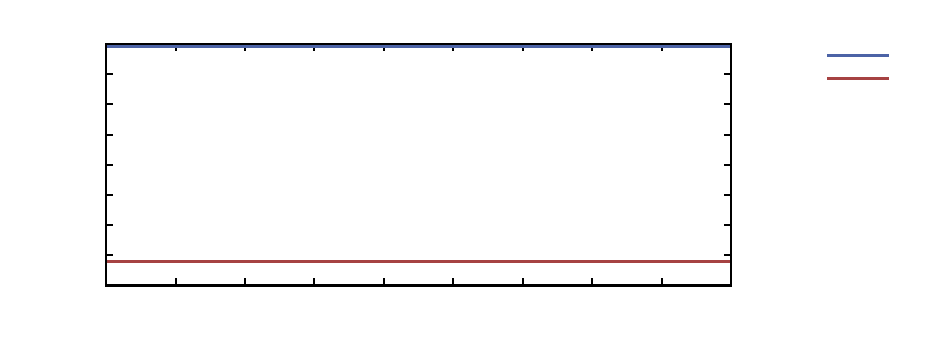
\includegraphics{memlog-systemd-without-vm}}%
    \gplfronttext
  \end{picture}%
\endgroup

  \caption {Systemd 의 메모리 기록 (가상 메모리 크기 제외)}
  \label{fig:systemd}
\end {figure}

\newpage
\subsection{memory-intensive 한 프로세스 - firefox}
Firefox 의 경우, 웹 페이지를 로드하고, 방문한 페이지 중 일부를 빠른 접근을 위해 메모리에 캐시하고, 자바스크립트를 구동하고, DOM 이벤트를 처리하는 등의 역활을 한다. 이는 동작하면서 많은 메모리를 사용하고, 더불어 잦은 메모리 크기의 변동이 발생할 것을 의미한다. 또한, 이 메모리 변화량의 대부분은, 함수 콜을 통한 스택에 위치하기보다는, heap에 위치하게 된다.

\begin {figure}[h]
  \centering
  % GNUPLOT: LaTeX picture with Postscript
\begingroup
  \makeatletter
  \providecommand\color[2][]{%
    \GenericError{(gnuplot) \space\space\space\@spaces}{%
      Package color not loaded in conjunction with
      terminal option `colourtext'%
    }{See the gnuplot documentation for explanation.%
    }{Either use 'blacktext' in gnuplot or load the package
      color.sty in LaTeX.}%
    \renewcommand\color[2][]{}%
  }%
  \providecommand\includegraphics[2][]{%
    \GenericError{(gnuplot) \space\space\space\@spaces}{%
      Package graphicx or graphics not loaded%
    }{See the gnuplot documentation for explanation.%
    }{The gnuplot epslatex terminal needs graphicx.sty or graphics.sty.}%
    \renewcommand\includegraphics[2][]{}%
  }%
  \providecommand\rotatebox[2]{#2}%
  \@ifundefined{ifGPcolor}{%
    \newif\ifGPcolor
    \GPcolortrue
  }{}%
  \@ifundefined{ifGPblacktext}{%
    \newif\ifGPblacktext
    \GPblacktextfalse
  }{}%
  % define a \g@addto@macro without @ in the name:
  \let\gplgaddtomacro\g@addto@macro
  % define empty templates for all commands taking text:
  \gdef\gplbacktext{}%
  \gdef\gplfronttext{}%
  \makeatother
  \ifGPblacktext
    % no textcolor at all
    \def\colorrgb#1{}%
    \def\colorgray#1{}%
  \else
    % gray or color?
    \ifGPcolor
      \def\colorrgb#1{\color[rgb]{#1}}%
      \def\colorgray#1{\color[gray]{#1}}%
      \expandafter\def\csname LTw\endcsname{\color{white}}%
      \expandafter\def\csname LTb\endcsname{\color{black}}%
      \expandafter\def\csname LTa\endcsname{\color{black}}%
      \expandafter\def\csname LT0\endcsname{\color[rgb]{1,0,0}}%
      \expandafter\def\csname LT1\endcsname{\color[rgb]{0,1,0}}%
      \expandafter\def\csname LT2\endcsname{\color[rgb]{0,0,1}}%
      \expandafter\def\csname LT3\endcsname{\color[rgb]{1,0,1}}%
      \expandafter\def\csname LT4\endcsname{\color[rgb]{0,1,1}}%
      \expandafter\def\csname LT5\endcsname{\color[rgb]{1,1,0}}%
      \expandafter\def\csname LT6\endcsname{\color[rgb]{0,0,0}}%
      \expandafter\def\csname LT7\endcsname{\color[rgb]{1,0.3,0}}%
      \expandafter\def\csname LT8\endcsname{\color[rgb]{0.5,0.5,0.5}}%
    \else
      % gray
      \def\colorrgb#1{\color{black}}%
      \def\colorgray#1{\color[gray]{#1}}%
      \expandafter\def\csname LTw\endcsname{\color{white}}%
      \expandafter\def\csname LTb\endcsname{\color{black}}%
      \expandafter\def\csname LTa\endcsname{\color{black}}%
      \expandafter\def\csname LT0\endcsname{\color{black}}%
      \expandafter\def\csname LT1\endcsname{\color{black}}%
      \expandafter\def\csname LT2\endcsname{\color{black}}%
      \expandafter\def\csname LT3\endcsname{\color{black}}%
      \expandafter\def\csname LT4\endcsname{\color{black}}%
      \expandafter\def\csname LT5\endcsname{\color{black}}%
      \expandafter\def\csname LT6\endcsname{\color{black}}%
      \expandafter\def\csname LT7\endcsname{\color{black}}%
      \expandafter\def\csname LT8\endcsname{\color{black}}%
    \fi
  \fi
    \setlength{\unitlength}{0.0500bp}%
    \ifx\gptboxheight\undefined%
      \newlength{\gptboxheight}%
      \newlength{\gptboxwidth}%
      \newsavebox{\gptboxtext}%
    \fi%
    \setlength{\fboxrule}{0.5pt}%
    \setlength{\fboxsep}{1pt}%
\begin{picture}(8640.00,3024.00)%
    \gplgaddtomacro\gplbacktext{%
      \csname LTb\endcsname%
      \put(1122,440){\makebox(0,0)[r]{\strut{}$0$}}%
      \put(1122,698){\makebox(0,0)[r]{\strut{}$200000$}}%
      \put(1122,955){\makebox(0,0)[r]{\strut{}$400000$}}%
      \put(1122,1213){\makebox(0,0)[r]{\strut{}$600000$}}%
      \put(1122,1471){\makebox(0,0)[r]{\strut{}$800000$}}%
      \put(1122,1728){\makebox(0,0)[r]{\strut{}$1\times10^{6}$}}%
      \put(1122,1986){\makebox(0,0)[r]{\strut{}$1.2\times10^{6}$}}%
      \put(1122,2244){\makebox(0,0)[r]{\strut{}$1.4\times10^{6}$}}%
      \put(1122,2501){\makebox(0,0)[r]{\strut{}$1.6\times10^{6}$}}%
      \put(1122,2759){\makebox(0,0)[r]{\strut{}$1.8\times10^{6}$}}%
      \put(1254,220){\makebox(0,0){\strut{}$0$}}%
      \put(1847,220){\makebox(0,0){\strut{}$20000$}}%
      \put(2441,220){\makebox(0,0){\strut{}$40000$}}%
      \put(3034,220){\makebox(0,0){\strut{}$60000$}}%
      \put(3628,220){\makebox(0,0){\strut{}$80000$}}%
      \put(4221,220){\makebox(0,0){\strut{}$100000$}}%
      \put(4815,220){\makebox(0,0){\strut{}$120000$}}%
      \put(5408,220){\makebox(0,0){\strut{}$140000$}}%
      \put(6002,220){\makebox(0,0){\strut{}$160000$}}%
      \put(6595,220){\makebox(0,0){\strut{}$180000$}}%
    }%
    \gplgaddtomacro\gplfronttext{%
      \csname LTb\endcsname%
      \put(7651,2649){\makebox(0,0)[r]{\strut{}size}}%
      \csname LTb\endcsname%
      \put(7651,2429){\makebox(0,0)[r]{\strut{}Rss}}%
      \csname LTb\endcsname%
      \put(7651,2209){\makebox(0,0)[r]{\strut{}shared}}%
    }%
    \gplbacktext
    \put(0,0){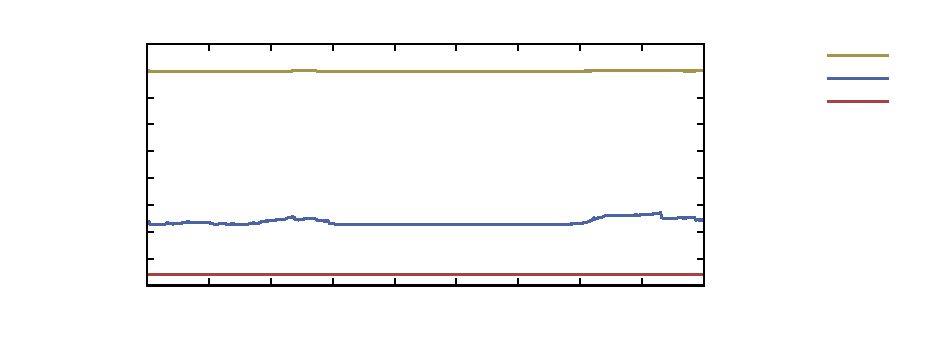
\includegraphics{memlog-firefox-with-vm}}%
    \gplfronttext
  \end{picture}%
\endgroup

  \caption {Firefox 의 메모리 기록}
  % GNUPLOT: LaTeX picture with Postscript
\begingroup
  \makeatletter
  \providecommand\color[2][]{%
    \GenericError{(gnuplot) \space\space\space\@spaces}{%
      Package color not loaded in conjunction with
      terminal option `colourtext'%
    }{See the gnuplot documentation for explanation.%
    }{Either use 'blacktext' in gnuplot or load the package
      color.sty in LaTeX.}%
    \renewcommand\color[2][]{}%
  }%
  \providecommand\includegraphics[2][]{%
    \GenericError{(gnuplot) \space\space\space\@spaces}{%
      Package graphicx or graphics not loaded%
    }{See the gnuplot documentation for explanation.%
    }{The gnuplot epslatex terminal needs graphicx.sty or graphics.sty.}%
    \renewcommand\includegraphics[2][]{}%
  }%
  \providecommand\rotatebox[2]{#2}%
  \@ifundefined{ifGPcolor}{%
    \newif\ifGPcolor
    \GPcolortrue
  }{}%
  \@ifundefined{ifGPblacktext}{%
    \newif\ifGPblacktext
    \GPblacktextfalse
  }{}%
  % define a \g@addto@macro without @ in the name:
  \let\gplgaddtomacro\g@addto@macro
  % define empty templates for all commands taking text:
  \gdef\gplbacktext{}%
  \gdef\gplfronttext{}%
  \makeatother
  \ifGPblacktext
    % no textcolor at all
    \def\colorrgb#1{}%
    \def\colorgray#1{}%
  \else
    % gray or color?
    \ifGPcolor
      \def\colorrgb#1{\color[rgb]{#1}}%
      \def\colorgray#1{\color[gray]{#1}}%
      \expandafter\def\csname LTw\endcsname{\color{white}}%
      \expandafter\def\csname LTb\endcsname{\color{black}}%
      \expandafter\def\csname LTa\endcsname{\color{black}}%
      \expandafter\def\csname LT0\endcsname{\color[rgb]{1,0,0}}%
      \expandafter\def\csname LT1\endcsname{\color[rgb]{0,1,0}}%
      \expandafter\def\csname LT2\endcsname{\color[rgb]{0,0,1}}%
      \expandafter\def\csname LT3\endcsname{\color[rgb]{1,0,1}}%
      \expandafter\def\csname LT4\endcsname{\color[rgb]{0,1,1}}%
      \expandafter\def\csname LT5\endcsname{\color[rgb]{1,1,0}}%
      \expandafter\def\csname LT6\endcsname{\color[rgb]{0,0,0}}%
      \expandafter\def\csname LT7\endcsname{\color[rgb]{1,0.3,0}}%
      \expandafter\def\csname LT8\endcsname{\color[rgb]{0.5,0.5,0.5}}%
    \else
      % gray
      \def\colorrgb#1{\color{black}}%
      \def\colorgray#1{\color[gray]{#1}}%
      \expandafter\def\csname LTw\endcsname{\color{white}}%
      \expandafter\def\csname LTb\endcsname{\color{black}}%
      \expandafter\def\csname LTa\endcsname{\color{black}}%
      \expandafter\def\csname LT0\endcsname{\color{black}}%
      \expandafter\def\csname LT1\endcsname{\color{black}}%
      \expandafter\def\csname LT2\endcsname{\color{black}}%
      \expandafter\def\csname LT3\endcsname{\color{black}}%
      \expandafter\def\csname LT4\endcsname{\color{black}}%
      \expandafter\def\csname LT5\endcsname{\color{black}}%
      \expandafter\def\csname LT6\endcsname{\color{black}}%
      \expandafter\def\csname LT7\endcsname{\color{black}}%
      \expandafter\def\csname LT8\endcsname{\color{black}}%
    \fi
  \fi
    \setlength{\unitlength}{0.0500bp}%
    \ifx\gptboxheight\undefined%
      \newlength{\gptboxheight}%
      \newlength{\gptboxwidth}%
      \newsavebox{\gptboxtext}%
    \fi%
    \setlength{\fboxrule}{0.5pt}%
    \setlength{\fboxsep}{1pt}%
\begin{picture}(8640.00,3024.00)%
    \gplgaddtomacro\gplbacktext{%
      \csname LTb\endcsname%
      \put(990,440){\makebox(0,0)[r]{\strut{}$50000$}}%
      \put(990,672){\makebox(0,0)[r]{\strut{}$100000$}}%
      \put(990,904){\makebox(0,0)[r]{\strut{}$150000$}}%
      \put(990,1136){\makebox(0,0)[r]{\strut{}$200000$}}%
      \put(990,1368){\makebox(0,0)[r]{\strut{}$250000$}}%
      \put(990,1600){\makebox(0,0)[r]{\strut{}$300000$}}%
      \put(990,1831){\makebox(0,0)[r]{\strut{}$350000$}}%
      \put(990,2063){\makebox(0,0)[r]{\strut{}$400000$}}%
      \put(990,2295){\makebox(0,0)[r]{\strut{}$450000$}}%
      \put(990,2527){\makebox(0,0)[r]{\strut{}$500000$}}%
      \put(990,2759){\makebox(0,0)[r]{\strut{}$550000$}}%
      \put(1122,220){\makebox(0,0){\strut{}$0$}}%
      \put(1759,220){\makebox(0,0){\strut{}$20000$}}%
      \put(2397,220){\makebox(0,0){\strut{}$40000$}}%
      \put(3034,220){\makebox(0,0){\strut{}$60000$}}%
      \put(3672,220){\makebox(0,0){\strut{}$80000$}}%
      \put(4309,220){\makebox(0,0){\strut{}$100000$}}%
      \put(4947,220){\makebox(0,0){\strut{}$120000$}}%
      \put(5584,220){\makebox(0,0){\strut{}$140000$}}%
      \put(6222,220){\makebox(0,0){\strut{}$160000$}}%
      \put(6859,220){\makebox(0,0){\strut{}$180000$}}%
    }%
    \gplgaddtomacro\gplfronttext{%
      \csname LTb\endcsname%
      \put(7651,2649){\makebox(0,0)[r]{\strut{}size}}%
      \csname LTb\endcsname%
      \put(7651,2429){\makebox(0,0)[r]{\strut{}Rss}}%
    }%
    \gplbacktext
    \put(0,0){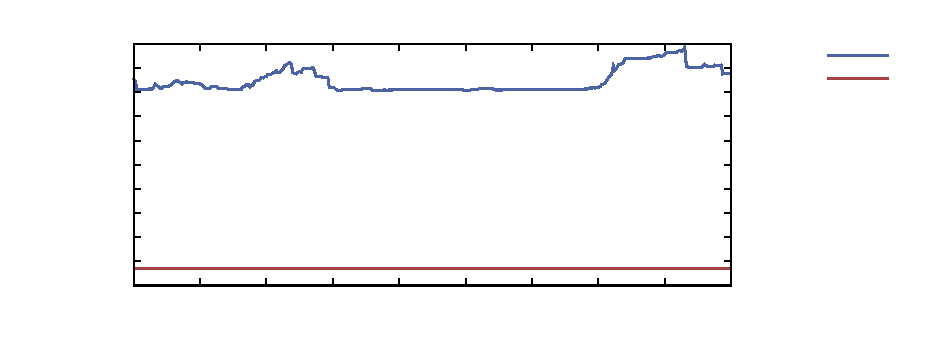
\includegraphics{memlog-firefox-without-vm}}%
    \gplfronttext
  \end{picture}%
\endgroup

  \caption {Firefox 의 메모리 기록 (가상 메모리 크기 제외)}
  \label{fig:firefox}
\end {figure}

\newpage
\subsection{기타 프로세스 - emacs}
Emacs 의 경우, 텍스트 버퍼와, lisp 실행을 제외하면, 메모리 변화가 적은 상황이다. 실제 결과에서, Rss 의 크기는, elisp 이 실행되고, 텍스트 버퍼의 내용이 변할 때만 변하는 것으로 나타났으며, Firefox 의 경우에 비해 매우 작은 메모리 사용량 변화를 나타내었다.

\begin {figure}[h]
  \centering
  % GNUPLOT: LaTeX picture with Postscript
\begingroup
  \makeatletter
  \providecommand\color[2][]{%
    \GenericError{(gnuplot) \space\space\space\@spaces}{%
      Package color not loaded in conjunction with
      terminal option `colourtext'%
    }{See the gnuplot documentation for explanation.%
    }{Either use 'blacktext' in gnuplot or load the package
      color.sty in LaTeX.}%
    \renewcommand\color[2][]{}%
  }%
  \providecommand\includegraphics[2][]{%
    \GenericError{(gnuplot) \space\space\space\@spaces}{%
      Package graphicx or graphics not loaded%
    }{See the gnuplot documentation for explanation.%
    }{The gnuplot epslatex terminal needs graphicx.sty or graphics.sty.}%
    \renewcommand\includegraphics[2][]{}%
  }%
  \providecommand\rotatebox[2]{#2}%
  \@ifundefined{ifGPcolor}{%
    \newif\ifGPcolor
    \GPcolortrue
  }{}%
  \@ifundefined{ifGPblacktext}{%
    \newif\ifGPblacktext
    \GPblacktextfalse
  }{}%
  % define a \g@addto@macro without @ in the name:
  \let\gplgaddtomacro\g@addto@macro
  % define empty templates for all commands taking text:
  \gdef\gplbacktext{}%
  \gdef\gplfronttext{}%
  \makeatother
  \ifGPblacktext
    % no textcolor at all
    \def\colorrgb#1{}%
    \def\colorgray#1{}%
  \else
    % gray or color?
    \ifGPcolor
      \def\colorrgb#1{\color[rgb]{#1}}%
      \def\colorgray#1{\color[gray]{#1}}%
      \expandafter\def\csname LTw\endcsname{\color{white}}%
      \expandafter\def\csname LTb\endcsname{\color{black}}%
      \expandafter\def\csname LTa\endcsname{\color{black}}%
      \expandafter\def\csname LT0\endcsname{\color[rgb]{1,0,0}}%
      \expandafter\def\csname LT1\endcsname{\color[rgb]{0,1,0}}%
      \expandafter\def\csname LT2\endcsname{\color[rgb]{0,0,1}}%
      \expandafter\def\csname LT3\endcsname{\color[rgb]{1,0,1}}%
      \expandafter\def\csname LT4\endcsname{\color[rgb]{0,1,1}}%
      \expandafter\def\csname LT5\endcsname{\color[rgb]{1,1,0}}%
      \expandafter\def\csname LT6\endcsname{\color[rgb]{0,0,0}}%
      \expandafter\def\csname LT7\endcsname{\color[rgb]{1,0.3,0}}%
      \expandafter\def\csname LT8\endcsname{\color[rgb]{0.5,0.5,0.5}}%
    \else
      % gray
      \def\colorrgb#1{\color{black}}%
      \def\colorgray#1{\color[gray]{#1}}%
      \expandafter\def\csname LTw\endcsname{\color{white}}%
      \expandafter\def\csname LTb\endcsname{\color{black}}%
      \expandafter\def\csname LTa\endcsname{\color{black}}%
      \expandafter\def\csname LT0\endcsname{\color{black}}%
      \expandafter\def\csname LT1\endcsname{\color{black}}%
      \expandafter\def\csname LT2\endcsname{\color{black}}%
      \expandafter\def\csname LT3\endcsname{\color{black}}%
      \expandafter\def\csname LT4\endcsname{\color{black}}%
      \expandafter\def\csname LT5\endcsname{\color{black}}%
      \expandafter\def\csname LT6\endcsname{\color{black}}%
      \expandafter\def\csname LT7\endcsname{\color{black}}%
      \expandafter\def\csname LT8\endcsname{\color{black}}%
    \fi
  \fi
    \setlength{\unitlength}{0.0500bp}%
    \ifx\gptboxheight\undefined%
      \newlength{\gptboxheight}%
      \newlength{\gptboxwidth}%
      \newsavebox{\gptboxtext}%
    \fi%
    \setlength{\fboxrule}{0.5pt}%
    \setlength{\fboxsep}{1pt}%
\begin{picture}(8640.00,3024.00)%
    \gplgaddtomacro\gplbacktext{%
      \csname LTb\endcsname%
      \put(990,440){\makebox(0,0)[r]{\strut{}$0$}}%
      \put(990,771){\makebox(0,0)[r]{\strut{}$100000$}}%
      \put(990,1103){\makebox(0,0)[r]{\strut{}$200000$}}%
      \put(990,1434){\makebox(0,0)[r]{\strut{}$300000$}}%
      \put(990,1765){\makebox(0,0)[r]{\strut{}$400000$}}%
      \put(990,2096){\makebox(0,0)[r]{\strut{}$500000$}}%
      \put(990,2428){\makebox(0,0)[r]{\strut{}$600000$}}%
      \put(990,2759){\makebox(0,0)[r]{\strut{}$700000$}}%
      \put(1122,220){\makebox(0,0){\strut{}$0$}}%
      \put(1730,220){\makebox(0,0){\strut{}$20000$}}%
      \put(2338,220){\makebox(0,0){\strut{}$40000$}}%
      \put(2946,220){\makebox(0,0){\strut{}$60000$}}%
      \put(3554,220){\makebox(0,0){\strut{}$80000$}}%
      \put(4163,220){\makebox(0,0){\strut{}$100000$}}%
      \put(4771,220){\makebox(0,0){\strut{}$120000$}}%
      \put(5379,220){\makebox(0,0){\strut{}$140000$}}%
      \put(5987,220){\makebox(0,0){\strut{}$160000$}}%
      \put(6595,220){\makebox(0,0){\strut{}$180000$}}%
    }%
    \gplgaddtomacro\gplfronttext{%
      \csname LTb\endcsname%
      \put(7651,2649){\makebox(0,0)[r]{\strut{}size}}%
      \csname LTb\endcsname%
      \put(7651,2429){\makebox(0,0)[r]{\strut{}Rss}}%
      \csname LTb\endcsname%
      \put(7651,2209){\makebox(0,0)[r]{\strut{}shared}}%
    }%
    \gplbacktext
    \put(0,0){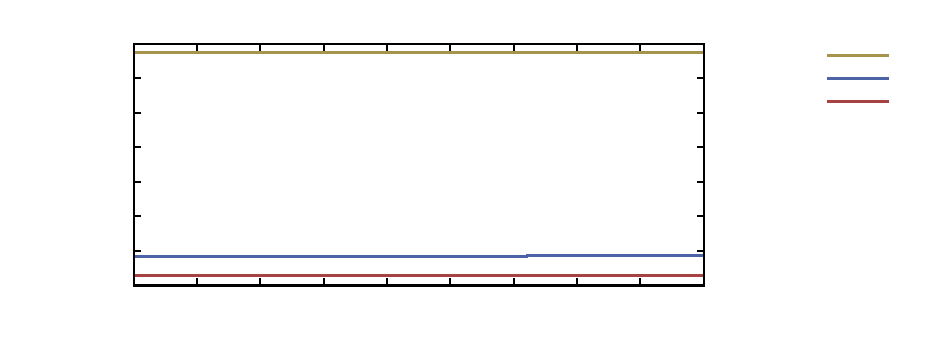
\includegraphics{memlog-emacs-with-vm}}%
    \gplfronttext
  \end{picture}%
\endgroup

  \caption {Emacs 의 메모리 기록}
  % GNUPLOT: LaTeX picture with Postscript
\begingroup
  \makeatletter
  \providecommand\color[2][]{%
    \GenericError{(gnuplot) \space\space\space\@spaces}{%
      Package color not loaded in conjunction with
      terminal option `colourtext'%
    }{See the gnuplot documentation for explanation.%
    }{Either use 'blacktext' in gnuplot or load the package
      color.sty in LaTeX.}%
    \renewcommand\color[2][]{}%
  }%
  \providecommand\includegraphics[2][]{%
    \GenericError{(gnuplot) \space\space\space\@spaces}{%
      Package graphicx or graphics not loaded%
    }{See the gnuplot documentation for explanation.%
    }{The gnuplot epslatex terminal needs graphicx.sty or graphics.sty.}%
    \renewcommand\includegraphics[2][]{}%
  }%
  \providecommand\rotatebox[2]{#2}%
  \@ifundefined{ifGPcolor}{%
    \newif\ifGPcolor
    \GPcolortrue
  }{}%
  \@ifundefined{ifGPblacktext}{%
    \newif\ifGPblacktext
    \GPblacktextfalse
  }{}%
  % define a \g@addto@macro without @ in the name:
  \let\gplgaddtomacro\g@addto@macro
  % define empty templates for all commands taking text:
  \gdef\gplbacktext{}%
  \gdef\gplfronttext{}%
  \makeatother
  \ifGPblacktext
    % no textcolor at all
    \def\colorrgb#1{}%
    \def\colorgray#1{}%
  \else
    % gray or color?
    \ifGPcolor
      \def\colorrgb#1{\color[rgb]{#1}}%
      \def\colorgray#1{\color[gray]{#1}}%
      \expandafter\def\csname LTw\endcsname{\color{white}}%
      \expandafter\def\csname LTb\endcsname{\color{black}}%
      \expandafter\def\csname LTa\endcsname{\color{black}}%
      \expandafter\def\csname LT0\endcsname{\color[rgb]{1,0,0}}%
      \expandafter\def\csname LT1\endcsname{\color[rgb]{0,1,0}}%
      \expandafter\def\csname LT2\endcsname{\color[rgb]{0,0,1}}%
      \expandafter\def\csname LT3\endcsname{\color[rgb]{1,0,1}}%
      \expandafter\def\csname LT4\endcsname{\color[rgb]{0,1,1}}%
      \expandafter\def\csname LT5\endcsname{\color[rgb]{1,1,0}}%
      \expandafter\def\csname LT6\endcsname{\color[rgb]{0,0,0}}%
      \expandafter\def\csname LT7\endcsname{\color[rgb]{1,0.3,0}}%
      \expandafter\def\csname LT8\endcsname{\color[rgb]{0.5,0.5,0.5}}%
    \else
      % gray
      \def\colorrgb#1{\color{black}}%
      \def\colorgray#1{\color[gray]{#1}}%
      \expandafter\def\csname LTw\endcsname{\color{white}}%
      \expandafter\def\csname LTb\endcsname{\color{black}}%
      \expandafter\def\csname LTa\endcsname{\color{black}}%
      \expandafter\def\csname LT0\endcsname{\color{black}}%
      \expandafter\def\csname LT1\endcsname{\color{black}}%
      \expandafter\def\csname LT2\endcsname{\color{black}}%
      \expandafter\def\csname LT3\endcsname{\color{black}}%
      \expandafter\def\csname LT4\endcsname{\color{black}}%
      \expandafter\def\csname LT5\endcsname{\color{black}}%
      \expandafter\def\csname LT6\endcsname{\color{black}}%
      \expandafter\def\csname LT7\endcsname{\color{black}}%
      \expandafter\def\csname LT8\endcsname{\color{black}}%
    \fi
  \fi
    \setlength{\unitlength}{0.0500bp}%
    \ifx\gptboxheight\undefined%
      \newlength{\gptboxheight}%
      \newlength{\gptboxwidth}%
      \newsavebox{\gptboxtext}%
    \fi%
    \setlength{\fboxrule}{0.5pt}%
    \setlength{\fboxsep}{1pt}%
\begin{picture}(8640.00,3024.00)%
    \gplgaddtomacro\gplbacktext{%
      \csname LTb\endcsname%
      \put(858,440){\makebox(0,0)[r]{\strut{}$30000$}}%
      \put(858,827){\makebox(0,0)[r]{\strut{}$40000$}}%
      \put(858,1213){\makebox(0,0)[r]{\strut{}$50000$}}%
      \put(858,1600){\makebox(0,0)[r]{\strut{}$60000$}}%
      \put(858,1986){\makebox(0,0)[r]{\strut{}$70000$}}%
      \put(858,2373){\makebox(0,0)[r]{\strut{}$80000$}}%
      \put(858,2759){\makebox(0,0)[r]{\strut{}$90000$}}%
      \put(990,220){\makebox(0,0){\strut{}$0$}}%
      \put(1642,220){\makebox(0,0){\strut{}$20000$}}%
      \put(2294,220){\makebox(0,0){\strut{}$40000$}}%
      \put(2946,220){\makebox(0,0){\strut{}$60000$}}%
      \put(3598,220){\makebox(0,0){\strut{}$80000$}}%
      \put(4251,220){\makebox(0,0){\strut{}$100000$}}%
      \put(4903,220){\makebox(0,0){\strut{}$120000$}}%
      \put(5555,220){\makebox(0,0){\strut{}$140000$}}%
      \put(6207,220){\makebox(0,0){\strut{}$160000$}}%
      \put(6859,220){\makebox(0,0){\strut{}$180000$}}%
    }%
    \gplgaddtomacro\gplfronttext{%
      \csname LTb\endcsname%
      \put(7651,2649){\makebox(0,0)[r]{\strut{}size}}%
      \csname LTb\endcsname%
      \put(7651,2429){\makebox(0,0)[r]{\strut{}Rss}}%
    }%
    \gplbacktext
    \put(0,0){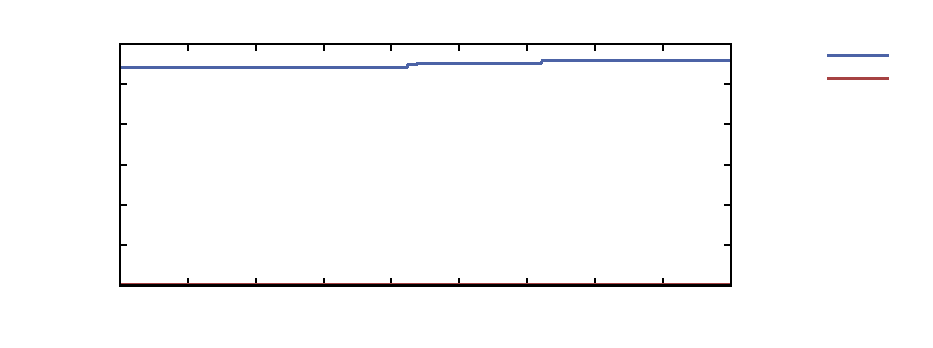
\includegraphics{memlog-emacs-without-vm}}%
    \gplfronttext
  \end{picture}%
\endgroup

  \caption {Emacs 의 메모리 기록 (가상 메모리 크기 제외)}
  \label{fig:emacs}
\end {figure}

\newpage
\section {Working set 의 추측}
Firefox 의 경우에서, Rss 의 증가량의 평균을 내어보면, 192KiB 정도가 나오게 된다. 이는 Working set 이 192KiB 정도일 때, Firefox 를 구동하는데, 페이징 폴트를 낮게 유지하며, 가동될 수 있음을 추측해 볼 수 있다.

\section {과제 중 발생한 문제점과 그 해결}
C99 에서 usleep() 이 지원되지 않아, 이를 지원하기 위해 GNU C99 dialect 로 컴파일 옵션을 바꾸어야 하는 일이 있었다.
\end {document}
